\documentclass[11pt,a4paper,oneside]{book}
%
%--------------------   start of the 'preamble'
%
\usepackage{graphicx,amssymb,amstext,amsmath,color,array,ctable,booktabs,wrapfig,caption}
%
\usepackage[table]{xcolor}
\usepackage{graphics}
\usepackage{hyperref}
\usepackage{pgf}

\usepackage{titlesec}
\titleformat{\chapter}[hang] 
{\normalfont\huge\bfseries}{\ \thechapter}{1em}{} 
\usepackage{tikz}
\usetikzlibrary{shapes}
\usetikzlibrary{calc,backgrounds}
\usetikzlibrary{automata}
\usetikzlibrary{arrows,positioning,calc,matrix} 
\usetikzlibrary{decorations.pathreplacing,shapes.multipart}

\tikzstyle{Dstate}=[shape=circle,draw=black!50,fill=black!10]
\tikzstyle{Istate}=[shape=diamond,draw=black!50,fill=black!10]
\tikzstyle{Mstate}=[shape=rectangle,draw=black!50,fill=black!10]

\tikzstyle{empty}=[shape=circle]

\tikzstyle{lightedge}=[->,dotted,thick]
\tikzstyle{mainstate}=[state,thick]
\tikzstyle{mainedge}=[->,thick]

%\renewcommand{\chaptername}{}
%\renewcommand{\thechapter}{}

\definecolor{black}{RGB}{0,0,0}
\definecolor{darkgrey}{RGB}{64,64,64}
\definecolor{grey}{RGB}{127,127,127}
\definecolor{lightgrey}{RGB}{230,230,230}

% scheme 1 
\definecolor{winered}{RGB}{158,16,0}
\definecolor{lightred}{RGB}{199,53,42}
\definecolor{brown}{RGB}{158,95,0}
\definecolor{orange}{RGB}{235,141,0}

%scheme2

\definecolor{darkblue}{RGB}{19,48,182}

\definecolor{blue}{RGB}{36,89,158}
\definecolor{browngreen}{RGB}{82,75,19}
\definecolor{lightbrown}{RGB}{158,126,36}

%scheme3

\definecolor{green}{RGB}{52,132,23}


\definecolor{lightgreen}{RGB}{82,209,36}
\definecolor{lightbrowngreen}{RGB}{125,133,23}
\definecolor{yellowgreen}{RGB}{198,209,36}

%scheme4


\definecolor{paper}{RGB}{240,238,183}
\definecolor{organicgrey}{RGB}{163,162,124}


\definecolor{metal}{RGB}{75,81,82}


\setlength{\parindent}{0cm}
\pagestyle{empty}

\makeindex
\usepackage{anysize}

%\marginsize{left}{right}{top}{bottom}:
\marginsize{2cm}{2cm}{2cm}{2cm}

\newcommand{\aln}[2]{\shortstack{ #1\\  #2}}

\begin{document}
\frontmatter
%-----------------------------------------------------------
\newlength{\centeroffset}
%\setlength{\centeroffset}{-0.5\oddsidemargin}
%\addtolength{\centeroffset}{0.5\evensidemargin}
%\addtolength{\textwidth}{-\centeroffset}
\thispagestyle{empty}
\vspace*{\stretch{1}}
\noindent\hspace*{\centeroffset}\makebox[0pt][l]{\begin{minipage}{\textwidth}
\flushright
{\Huge\bfseries 

The TagDust2 Manual

}


\end{minipage}}

\vspace{\stretch{1}}
\noindent\hspace*{\centeroffset}\makebox[0pt][l]{\begin{minipage}{\textwidth}
\flushright


\vspace{\stretch{1}}
{\bfseries 
by Timo Lassmann\\[1.5ex]} 
\noindent\rule[-1ex]{\textwidth}{1pt}\\[2.5ex]
 \today

\end{minipage}}

%\addtolength{\textwidth}{\centeroffset}
%\vspace{\stretch{2}}


\pagebreak
\begin{small} 

Copyright \copyright 2013 Timo Lassmann (timolassmann@gmail.com)
 
 This document is free;  you can redistribute it and/or modify
 it under the terms of the GNU General Public License as published by
 the Free Software Foundation, either version 3 of the License, or
 (at your option) any later version.
 
 This document is distributed in the hope that it will be useful,
 but WITHOUT ANY WARRANTY; without even the implied warranty of
 MERCHANTABILITY or FITNESS FOR A PARTICULAR PURPOSE.  See the
 GNU General Public License for more details.
 
 You should have received a copy of the GNU General Public License
 along with TagDust.  
 
 If not, see (http://www.gnu.org/licenses/).



\end{small}

%-----------------------------------------------------------
\tableofcontents
%-----------------------------------------------------------
\mainmatter
%\setcounter{chapter}{-1}

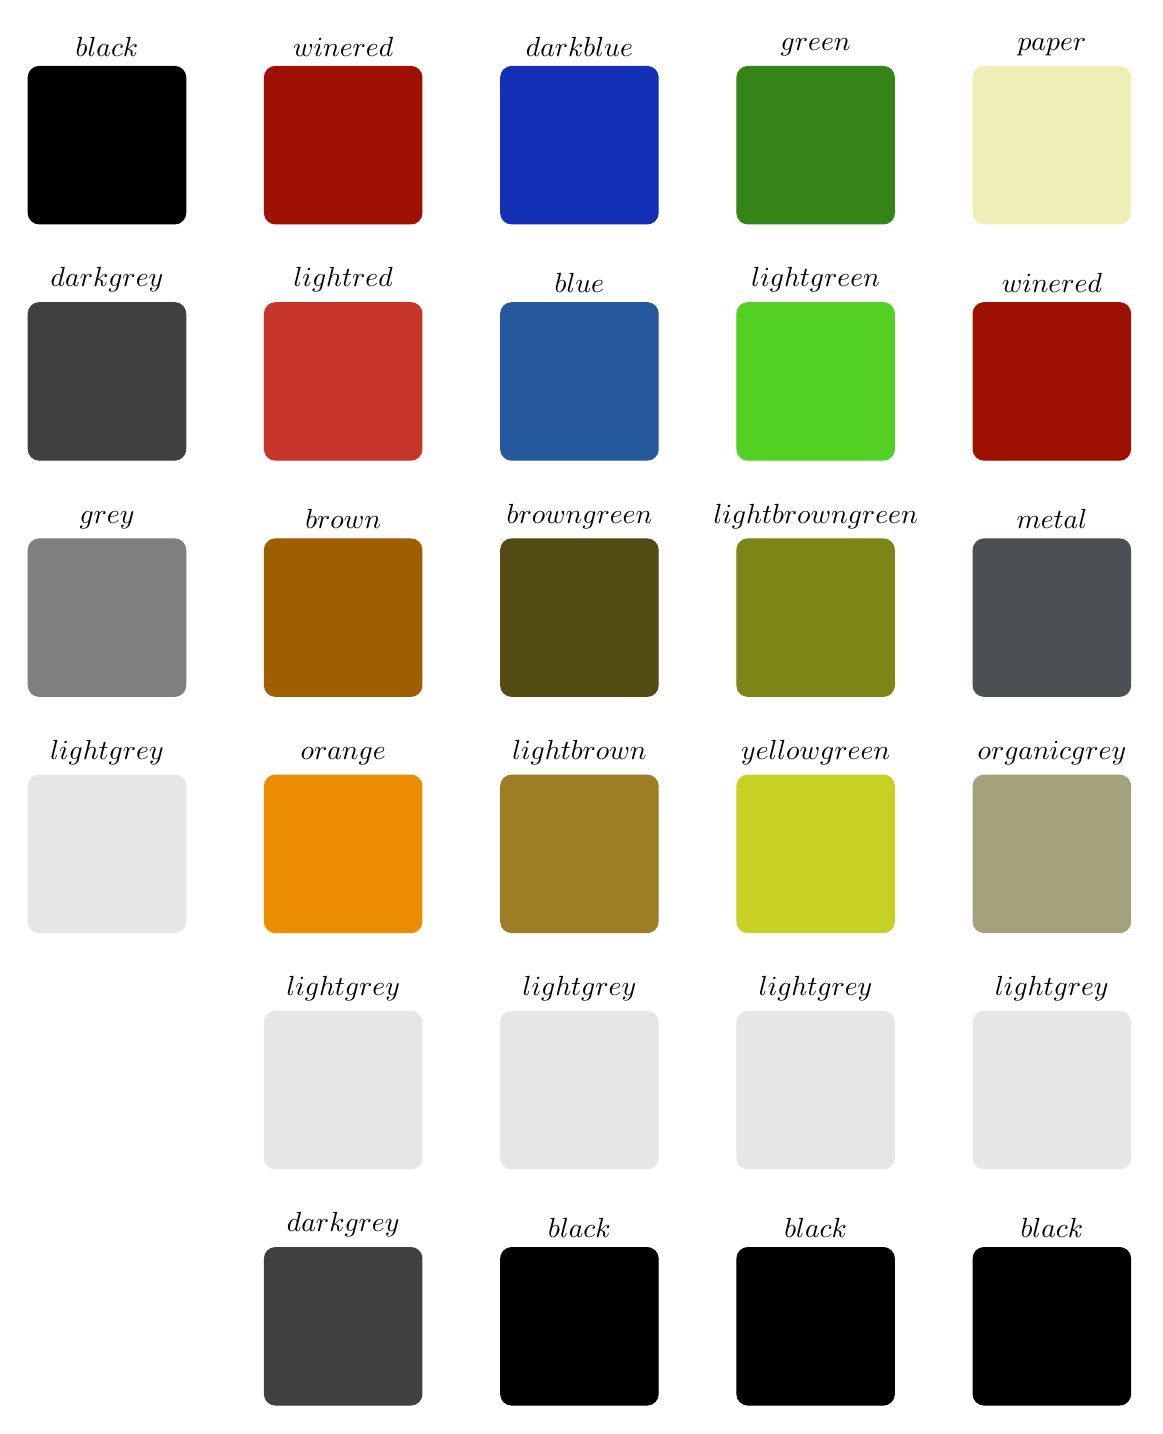
\begin{tikzpicture}[]
%\definecolor{black}{RGB}{0,0,0}
%\definecolor{darkgrey}{RGB}{64,64,64}
%\definecolor{grey}{RGB}{127,127,127}
%\definecolor{lightgrey}{RGB}{230,230,230}
\node [draw=black, fill=black,rounded corners=4pt,draw,rectangle,minimum width=2cm,minimum height=2cm,label=$black$] at (0,0) {};

\node [draw=darkgrey, fill=darkgrey,rounded corners=4pt,draw,rectangle,minimum width=2cm,minimum height=2cm,label=$darkgrey$] at (0,-3) {};

\node [draw=grey, fill=grey,rounded corners=4pt,draw,rectangle,minimum width=2cm,minimum height=2cm,label=$grey$] at (0,-6) {};

\node [draw=lightgrey, fill=lightgrey,rounded corners=4pt,draw,rectangle,minimum width=2cm,minimum height=2cm,label=$lightgrey$] at (0,-9) {};

%\definecolor{winered}{RGB}{158,16,0}
%\definecolor{ligthred}{RGB}{199,53,42}
%\definecolor{brown}{RGB}{158,95,0}
%\definecolor{orange}{RGB}{235,141,0}
\begin{scope}[shift={(3,0)}];
\node [draw=winered, fill=winered,rounded corners=4pt,draw,rectangle,minimum width=2cm,minimum height=2cm,label=$winered$] at (0,0) {};

\node [draw=lightred, fill=lightred,rounded corners=4pt,draw,rectangle,minimum width=2cm,minimum height=2cm,label=$lightred$] at (0,-3) {};

\node [draw=brown, fill=brown,rounded corners=4pt,draw,rectangle,minimum width=2cm,minimum height=2cm,label=$brown$] at (0,-6) {};

\node [draw=orange, fill=orange,rounded corners=4pt,draw,rectangle,minimum width=2cm,minimum height=2cm,label=$orange$] at (0,-9) {};

\node [draw=lightgrey, fill=lightgrey,rounded corners=4pt,draw,rectangle,minimum width=2cm,minimum height=2cm,label=$lightgrey$] at (0,-12) {};

\node [draw=darkgrey, fill=darkgrey,rounded corners=4pt,draw,rectangle,minimum width=2cm,minimum height=2cm,label=$darkgrey$] at (0,-15) {};

\end{scope}


%\definecolor{darkblue}{RGB}{19,48,182}

%\definecolor{blue}{RGB}{36,89,158}
%\definecolor{browngreen}{RGB}{82,75,19}
%\definecolor{lightbrown}{RGB}{158,126,36}

\begin{scope}[shift={(6,0)}];
\node [draw=darkblue, fill=darkblue,rounded corners=4pt,draw,rectangle,minimum width=2cm,minimum height=2cm,label=$darkblue$] at (0,0) {};

\node [draw=blue, fill=blue,rounded corners=4pt,draw,rectangle,minimum width=2cm,minimum height=2cm,label=$blue$] at (0,-3) {};

\node [draw=browngreen, fill=browngreen,rounded corners=4pt,draw,rectangle,minimum width=2cm,minimum height=2cm,label=$browngreen$] at (0,-6) {};

\node [draw=lightbrown, fill=lightbrown,rounded corners=4pt,draw,rectangle,minimum width=2cm,minimum height=2cm,label=$lightbrown$] at (0,-9) {};

\node [draw=lightgrey, fill=lightgrey,rounded corners=4pt,draw,rectangle,minimum width=2cm,minimum height=2cm,label=$lightgrey$] at (0,-12) {};

\node [draw=black, fill=black,rounded corners=4pt,draw,rectangle,minimum width=2cm,minimum height=2cm,label=$black$] at (0,-15) {};

\end{scope}

%\definecolor{green}{RGB}{52,132,23}
%\definecolor{lightgreen}{RGB}{82,209,36}
%\definecolor{lightbrowngreen}{RGB}{125,133,23}
%\definecolor{yellowgreen}{RGB}{198,209,36}


\begin{scope}[shift={(9,0)}];
\node [draw=green, fill=green,rounded corners=4pt,draw,rectangle,minimum width=2cm,minimum height=2cm,label=$green$] at (0,0) {};

\node [draw=lightgreen, fill=lightgreen,rounded corners=4pt,draw,rectangle,minimum width=2cm,minimum height=2cm,label=$lightgreen$] at (0,-3) {};

\node [draw=lightbrowngreen, fill=lightbrowngreen,rounded corners=4pt,draw,rectangle,minimum width=2cm,minimum height=2cm,label=$lightbrowngreen$] at (0,-6) {};

\node [draw=yellowgreen, fill=yellowgreen,rounded corners=4pt,draw,rectangle,minimum width=2cm,minimum height=2cm,label=$yellowgreen$] at (0,-9) {};

\node [draw=lightgrey, fill=lightgrey,rounded corners=4pt,draw,rectangle,minimum width=2cm,minimum height=2cm,label=$lightgrey$] at (0,-12) {};

\node [draw=black, fill=black,rounded corners=4pt,draw,rectangle,minimum width=2cm,minimum height=2cm,label=$black$] at (0,-15) {};

\end{scope}

%\definecolor{paper}{RGB}{240,238,183}
%\definecolor{organicgrey}{RGB}{163,162,124}
%\definecolor{metal}{RGB}{75,81,82}

\begin{scope}[shift={(12,0)}];
\node [draw=paper, fill=paper,rounded corners=4pt,draw,rectangle,minimum width=2cm,minimum height=2cm,label=$paper$] at (0,0) {};

\node [draw=winered, fill=winered,rounded corners=4pt,draw,rectangle,minimum width=2cm,minimum height=2cm,label=$winered$] at (0,-3) {};

\node [draw=metal, fill=metal,rounded corners=4pt,draw,rectangle,minimum width=2cm,minimum height=2cm,label=$metal$] at (0,-6) {};

\node [draw=organicgrey, fill=organicgrey,rounded corners=4pt,draw,rectangle,minimum width=2cm,minimum height=2cm,label=$organicgrey$] at (0,-9) {};

\node [draw=lightgrey, fill=lightgrey,rounded corners=4pt,draw,rectangle,minimum width=2cm,minimum height=2cm,label=$lightgrey$] at (0,-12) {};

\node [draw=black, fill=black,rounded corners=4pt,draw,rectangle,minimum width=2cm,minimum height=2cm,label=$black$] at (0,-15) {};


\end{scope}


%\draw[rounded corners=4pt,draw=hgrey, fill=hlightblue] (0,-6)	rectangle (+1,+1);
%\draw[rounded corners=4pt,draw=hgrey, fill=hlightblue] (0,-9)	rectangle (+1,+1);




\end{tikzpicture}
%\setcounter{chapter}{1}
%\setcounter{section}{0}
\chapter{Introduction}

 %\addcontentsline{toc}{chapter}{Introduction}

The raw sequences produced by next generation sequencing (NGS) machines contain linker sequences and barcode sequenced used to label samples. TagDust2 is a program to extract and label the sequences to be analyzed in downstream pipelines.

Tagdust allows users to specify the expected architecture of a read and converts it into a hidden Markov model. The latter can assign sequences to a particular barcode (or index) even in the presence of sequencing errors.


%\begin{wrapfigure}{l}{1\textwidth}

\begin{figure}[h]
 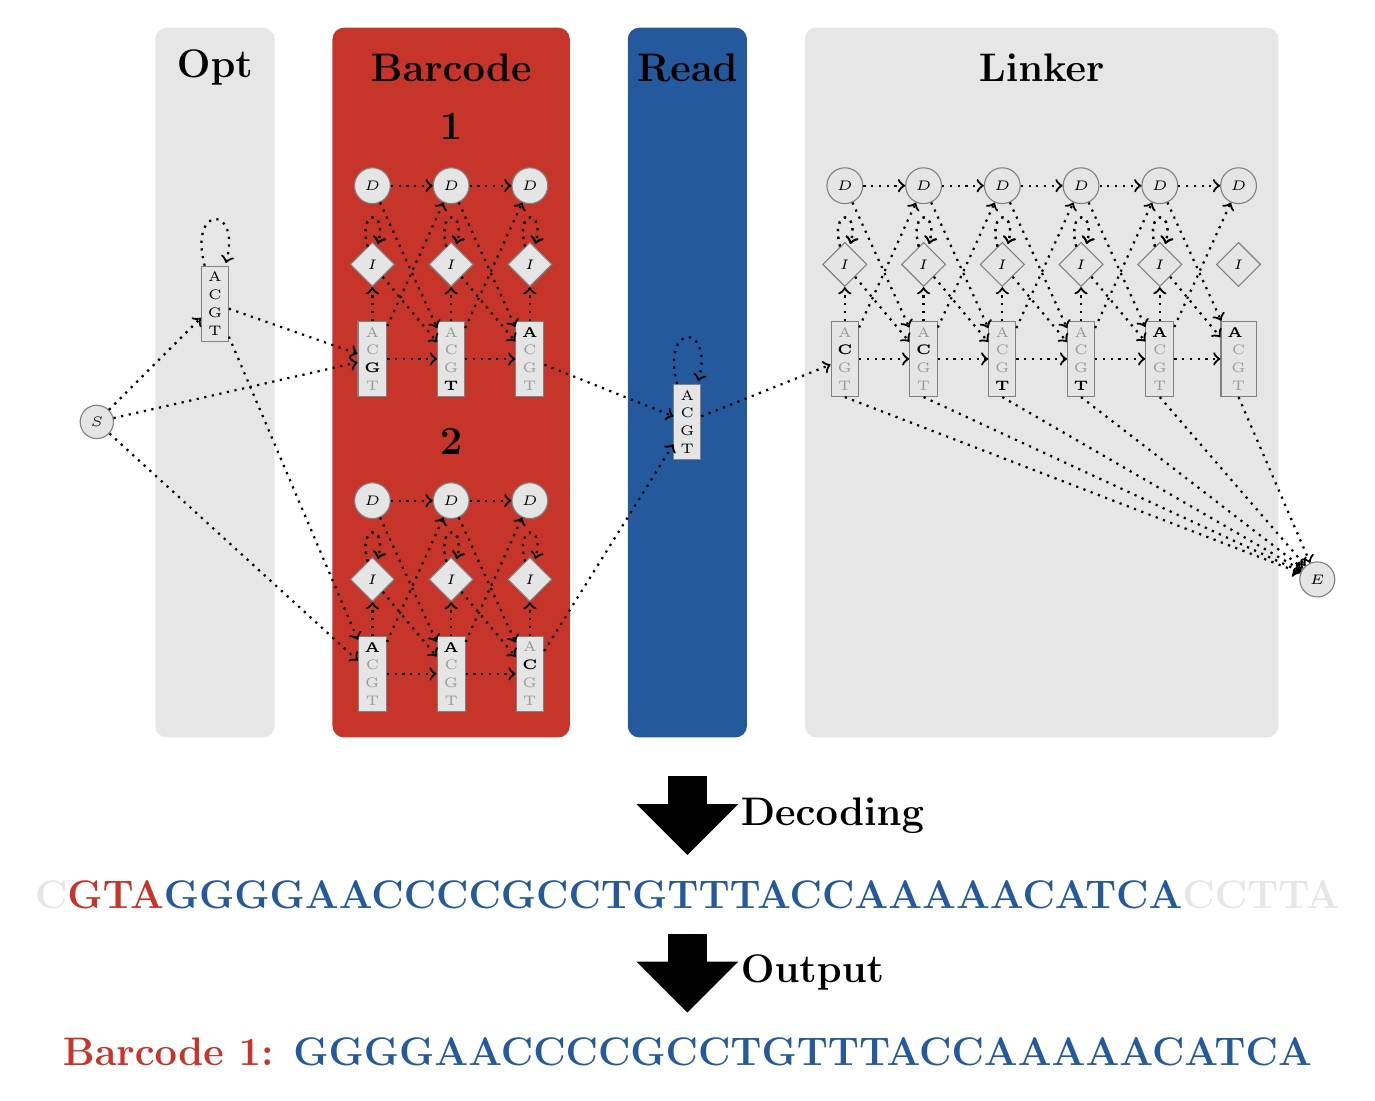
\begin{tikzpicture}[]
 \tiny

\draw[rounded corners=4pt,draw=lightgrey, fill=lightgrey] (-0.75,5)	rectangle (0.75,-4);

\draw[rounded corners=4pt,draw=lightred, fill=lightred] (1.5,5)	rectangle (4.5,-4);
 

\draw[rounded corners=4pt,draw=blue, fill=blue] (5.25,5)	rectangle (6.75,-4);
  
\draw[rounded corners=4pt,draw=lightgrey, fill=lightgrey] (7.5,5)	rectangle (13.5,-4);

 \node  at (0,4.5)  [font=\Large,style={align=center}] () {{\bf Opt}};
 
 \node  at (3,4.5)  [font=\Large,style={align=center}] () {{\bf Barcode}};
 
  \node  at (3,2+1.75)  [font=\Large,style={align=center}] () {{\bf 1}};
  
    \node  at (3,-2+ 1.75)  [font=\Large,style={align=center}] () {{\bf 2}};
  \node  at (6,4.5)  [font=\Large,style={align=center}] () {{\bf Read}};
  
    \node  at (10.5,4.5)  [font=\Large,style={align=center}] () {{\bf Linker}};
    
\draw[
        -triangle 90,
        line width=2mm,
        postaction={draw, line width=0.5cm, shorten >=0.5cm, -}
    ] (6,-4.5) -- node[right=0.5,font =\Large] {{\bf Decoding}} (6,-5.5) ;
    
  \node[draw=white, thick,font=\Large] at (6,-6)  {\bf {\color{lightgrey}C}{\color{lightred}GTA}{\color{blue}GGGGAACCCCGCCTGTTTACCAAAAACATCA}{\color{lightgrey}CCTTA}} ;
  
  \draw[
        -triangle 90,
        line width=2mm,
        postaction={draw, line width=0.5cm, shorten >=0.5cm, -}
    ] (6,-6.5) -- node[right=0.5,font =\Large] {{\bf Output}} (6,-7.5) ;
  
  \node[draw=white, thick,font=\Large] at (6,-8)  {\bf  {\color{lightred}Barcode 1:}  {\color{blue}GGGGAACCCCGCCTGTTTACCAAAAACATCA}} ;
  
  
\begin{scope}[shift={(-1.5,0)}];
\node[Dstate] (START) at (0,0){$S$};
\end{scope}

\begin{scope}[shift={(0,1.5)}];
\node[Mstate] (O1) at (0,0){\shortstack{ A\\   C\\  G\\ T} };
\end{scope}

\begin{scope}[shift={(2,2)}];
\node[Dstate] (d1) at (0,1){$D$};
\node[Istate] (i1) at (0,0){$I$};
\node[Mstate] (m1) at (0,-1.2){\shortstack{ {\color{black!40}A}\\   {\color{black!40}C}\\  {\bf G}\\   {\color{black!40}T}} };



\node[Dstate] (d2) at (1,1){$D$};
\node[Istate] (i2) at (1,0){$I$};
\node[Mstate] (m2) at (1,-1.2){\shortstack{ {\color{black!40}A}\\   {\color{black!40}C}\\   {\color{black!40}G}\\   {\bf T}} };


\node[Dstate] (d3) at (2,1){$D$};
\node[Istate] (i3) at (2,-0){$I$};
\node[Mstate] (m3) at (2,-1.2){\shortstack{ {\bf A}\\   {\color{black!40}C}\\   {\color{black!40}G}\\   {\color{black!40}T}} };
\end{scope}


\begin{scope}[shift={(2,-2)}];

\node[Dstate] (d4) at (0,1){$D$};
\node[Istate] (i4) at (0,0){$I$};
\node[Mstate] (m4) at (0,-1.2){\shortstack{ {\bf A}\\   {\color{black!40}C}\\   {\color{black!40}G}\\   {\color{black!40}T}} };



\node[Dstate] (d5) at (1,1){$D$};
\node[Istate] (i5) at (1,0){$I$};
\node[Mstate] (m5) at (1,-1.2){\shortstack{ {\bf A}\\   {\color{black!40}C}\\   {\color{black!40}G}\\   {\color{black!40}T}} };


\node[Dstate] (d6) at (2,1){$D$};
\node[Istate] (i6) at (2,-0){$I$};
\node[Mstate] (m6) at (2,-1.2){\shortstack{ {\color{black!40}A}\\   {\bf C}\\   {\color{black!40}G}\\   {\color{black!40}T}} };
\end{scope}



\begin{scope}[shift={(6,0)}];



\node[Mstate] (R1) at (0,0){\shortstack{ A\\  C \\ G \\   T} };
\end{scope}



\begin{scope}[shift={(8,2)}];

%CCTTAAGG
\node[Dstate] (dl1) at (0,1){$D$};
\node[Istate] (il1) at (0,0){$I$};
\node[Mstate] (ml1) at (0,-1.2){\shortstack{ {\color{black!40}A}\\  {\bf C} \\   {\color{black!40}G}\\ {\color{black!40}T}} };



\node[Dstate] (dl2) at (1,1){$D$};
\node[Istate] (il2) at (1,0){$I$};
\node[Mstate] (ml2) at (1,-1.2){\shortstack{ {\color{black!40}A}\\   {\bf C}\\   {\color{black!40}G}\\   {\color{black!40}T}} };


\node[Dstate] (dl3) at (2,1){$D$};
\node[Istate] (il3) at (2,-0){$I$};
\node[Mstate] (ml3) at (2,-1.2){\shortstack{ {\color{black!40}A}\\   {\color{black!40}C}\\   {\color{black!40}G}\\   {\bf T}} };

\node[Dstate] (dl4) at (3,1){$D$};
\node[Istate] (il4) at (3,0){$I$};
\node[Mstate] (ml4) at (3,-1.2){\shortstack{ {\color{black!40}A}\\   {\color{black!40}C}\\   {\color{black!40}G}\\   {\bf T}} };

\node[Dstate] (dl5) at (4,1){$D$};
\node[Istate] (il5) at (4,0){$I$};
\node[Mstate] (ml5) at (4,-1.2){\shortstack{ {\bf A}\\   {\color{black!40}C}\\   {\color{black!40}G}\\   {\color{black!40}T}} };
\node[Dstate] (dl6) at (5,1){$D$};
\node[Istate] (il6) at (5,-0){$I$};
\node[Mstate] (ml6) at (5,-1.2){\shortstack{ {\bf A } \\   {\color{black!40}C}\\   {\color{black!40}G}\\   {\color{black!40}T}} };
\end{scope}

\begin{scope}[shift={(14,-2)}];
\node[Dstate] (END) at (0,0){$E$};
\end{scope}

 \path 
 
(START) edge [lightedge] (O1)

(START) edge [lightedge] (m1)

(START) edge [lightedge] (m4)
 
(O1) edge [lightedge, loop above] ()
(R1) edge [lightedge, loop above] ()
    
(O1)edge [lightedge] (m1)
(O1)edge [lightedge] (m4)
(R1)edge [lightedge] (ml1)

(ml1.south)edge [lightedge] (END)
(ml2.south)edge [lightedge] (END)
(ml3.south)edge [lightedge] (END)
(ml4.south)edge [lightedge] (END)
(ml5.south)edge [lightedge] (END)
(ml6.south)edge [lightedge] (END)


(m3)edge [lightedge] (R1)
(m6)edge [lightedge] (R1)

(m1) edge [lightedge] (m2) 
(m1) edge [lightedge] (d2) 
(m1) edge [lightedge] (i1)
   
(i1) edge [lightedge,loop above] ()
(i1) edge  [lightedge] (m2)
(i1) edge [lightedge, loop above] ()
(d1) edge  [lightedge,->] (d2)
(d1) edge  [lightedge,->] (m2)

(m2) edge [lightedge] (m3) 
(m2) edge [lightedge] (d3) 
(m2) edge [lightedge] (i2)
   
(i2) edge [lightedge,loop above] ()
(i2) edge  [lightedge] (m3)
(i2) edge [lightedge, loop above] ()
(d2) edge  [lightedge,->] (d3)
(d2) edge  [lightedge,->] (m3)


(m3) edge [lightedge] (i3)
   
(i3) edge [lightedge,loop above] ()

(i3) edge [lightedge, loop above] ()


(m4) edge [lightedge] (m5) 
(m4) edge [lightedge] (d5) 
(m4) edge [lightedge] (i4)
   
(i4) edge [lightedge,loop above] ()
(i4) edge  [lightedge] (m5)
(i4) edge [lightedge, loop above] ()
(d4) edge  [lightedge,->] (d5)
(d4) edge  [lightedge,->] (m5)

(m5) edge [lightedge] (m6) 
(m5) edge [lightedge] (d6) 
(m5) edge [lightedge] (i5)
   
(i5) edge [lightedge,loop above] ()
(i5) edge  [lightedge] (m6)
(i5) edge [lightedge, loop above] ()
(d5) edge  [lightedge,->] (d6)
(d5) edge  [lightedge,->] (m6)


(m6) edge [lightedge] (i6)
   
(i6) edge [lightedge,loop above] ()


 
(ml1) edge [lightedge] (ml2) 
(ml1) edge [lightedge] (dl2) 
(ml1) edge [lightedge] (il1)
   
(il1) edge [lightedge,loop above] ()
(il1) edge  [lightedge] (ml2)
(il1) edge [lightedge, loop above] ()
(dl1) edge  [lightedge,->] (dl2)
(dl1) edge  [lightedge,->] (ml2)

(ml2) edge [lightedge] (ml3) 
(ml2) edge [lightedge] (dl3) 
(ml2) edge [lightedge] (il2)
   
(il2) edge [lightedge,loop above] ()
(il2) edge  [lightedge] (ml3)
(il2) edge [lightedge, loop above] ()
(dl2) edge  [lightedge,->] (dl3)
(dl2) edge  [lightedge,->] (ml3)


(ml3) edge [lightedge] (ml4) 
(ml3) edge [lightedge] (dl4) 
(ml3) edge [lightedge] (il3)
   
(il3) edge [lightedge,loop above] ()
(il3) edge  [lightedge] (ml4)
(il3) edge [lightedge, loop above] ()
(dl3) edge  [lightedge,->] (dl4)
(dl3) edge  [lightedge,->] (ml4)


(ml4) edge [lightedge] (ml5) 
(ml4) edge [lightedge] (dl5) 
(ml4) edge [lightedge] (il4)
   
(il4) edge [lightedge,loop above] ()
(il4) edge  [lightedge] (ml5)
(il4) edge [lightedge, loop above] ()
(dl4) edge  [lightedge,->] (dl5)
(dl4) edge  [lightedge,->] (ml5)



(ml5) edge [lightedge] (ml6) 
(ml5) edge [lightedge] (dl6) 
(ml5) edge [lightedge] (il5)
   
(il5) edge [lightedge,loop above] ()
(il5) edge  [lightedge] (ml6)
(il5) edge [lightedge, loop above] ()
(dl5) edge  [lightedge,->] (dl6)
(dl5) edge  [lightedge,->] (ml6)





    ;

\end{tikzpicture}
\caption{A HMM specifies the expected architecture of the raw sequence. After decoding sequences are segmented into the components of the architecture. Based on the segmentation, a barcode is assigned to each read and accessory sequences are trimmed.}
\end{figure}


%\end{wrapfigure}

\newpage

\chapter{Installation}
%\addcontentsline{toc}{chapter}{Installation}


\section*{Quick installation instructions}
\addcontentsline{toc}{section}{Quick installation instructions}


\chapter*{General Information}
\setcounter{chapter}{2}
\setcounter{section}{0}
\addcontentsline{toc}{chapter}{General Information}
  
\section{Usage}
\rule[1cm]{\textwidth}{1pt}

All commands are accessible by calling Delve first. For example: 

\begin{verbatim}
bash-3.1$ delve index genome.fa 
\end{verbatim}
 - builds an index of the genome.
\begin{verbatim}
bash-3.1$ delve aln alignments.sam genome.fa
\end{verbatim}
- aligns reads to the genome.\\

Concise help is given by calling Delve with a command but without arguments.

\section{Formats}
\rule[1cm]{\textwidth}{1pt}
Delve employs widely used file formats to make integration into existing pipelines easier.\\
\subsection{FASTA}
Delve expects the genome to be in a single file fasta format. Reads can also be supplied in fasta format but fastq is preferred.\\

\subsection{FASTQ}
When available the reads should be supplied in fastq\cite{Cock:2009p3196} format. The actual quality values are not used by Delve at this point but are parsed for downstream analysis to the SAM output files.\\  

\subsection{SAM / BAM}
Alignments are given in SAM\cite{Li:2009p24} format. For an intermediate SAM file we adopted the 'XA:Z:' tag for alternative hits used by BWA\cite{Li:2009p3} to indicate additional alignments for each read in one line. In brief, the XA tag lists for each hit the chromosome, position, CIGAR line and number of mismatches separated by ';'. \\
\subsection{BEDgraph / WIG}

A description of these formats can be found at the UCSC genome browser site: 
\begin{itemize} 
\item \href{http://genome.ucsc.edu/goldenPath/help/bedgraph.html}{BEDgraph}
\item \href{http://genome.ucsc.edu/goldenPath/help/wiggle.html}{WIG}
\end{itemize}


\chapter*{ {\color{blue} Commands}}
\setcounter{chapter}{3}
\setcounter{section}{0}
\addcontentsline{toc}{chapter}{Commands}
  
This section gives a detailed explanation of each of Delve's commands. 
  
\section{index}
\rule[1cm]{\textwidth}{1pt}

Delve occasionally needs to extract sequences from the genome. The index command creates the necessary files in the same directory as the input genome.\\

{\bf Usage:} delve index $<$genome.fa$>$


\section{seed}
\rule[1cm]{\textwidth}{1pt}
Seed finds short seed matches for input reads and verifies each hit with Myers bit-parallel dynamic programming algorithm\cite{Myers:1998p28}. The output is a SAM file with the top 18 hits for each sequence. At this stage hits are ranked based on the edit distance. The best hit is reported in the default SAM format while additional hits are given in the 'XA:Z:' tag.\\ 

{\bf Usage:} delve seed {\bf [options]} $<$reads.fq$>$ $<$genome.fa$>$\\

\rowcolors{1}{lightgrey}{white}

\begin{center}
\begin{tabular}{| l | l | p{12cm}|}
\hline
\rowcolor{blue} \textcolor{white}{\scshape Option}		&\textcolor{white}{\scshape Type}		&	\textcolor{white}{\scshape Description}\\ \hline
-l & INT & seed length [12] \\
-s & INT & step size [8] \\
-t & INT & number of threads [4]\\
-o & STR & output SAM file [STDOUT]\\
-as & STR & adds assembly infomation to SAM header [NA]\\
\hline
\end{tabular}
\end{center}

Longer seed lengths decreases the running time of Delve drastically risks missing hits.\\

Example of output format(one SAM line): 
{\small
\begin{verbatim}
chr1_31332794_31333336_0:0:0_0:0:0_1 0 chr1 31332794 20 * * 0 0
   ACATAGACTTCAAAACTCAAACCAAATATTTC !!!!!!!!!!!!!!!!!!!!!!!!!!!!!!!! NM:i:0 
   XA:Z:chr10,-109598328,32M,5;chr5,-156754108,32M,5;chr4,+27656642,32M,5;chrX,+146319453,32M;
\end{verbatim}
}


\newpage
\section{aln}
\rule[1cm]{\textwidth}{1pt}

The align option both estimates parameters for the pair-HMM and then uses the parameterized model to align all reads. The output file contains both the best and secondary alignments marked with the 0x100 SAM flag. In the rare case of two alignment having multiple equivalent mapping locations one is chosen at random and the others marked as secondary. To keep the output size manageable, only secondary alignments with a posterior probability of $\geq$ 0.1 are reported.\\ 

{\bf Usage:} delve aln {\bf [options]} $<$in.sam$>$ $<$genome.fa$>$\\

\rowcolors{1}{lightgrey}{white}

\begin{center}
\begin{tabular}{| l | l | p{12cm}|}
\hline
\rowcolor{blue} \textcolor{white}{\scshape Option}		&\textcolor{white}{\scshape Type}		&	\textcolor{white}{\scshape Description}\\ \hline
-m & STR & model file [off] \\
-t & INT & number of threads [8]\\
-o & STR & output SAM file [STDOUT]\\
-as & STR & adds assembly infomation to SAM header [NA]\\
\hline
\end{tabular}
\end{center}

The -m option has two functions: if no model exists the trained model parameters are written to file STR for future use otherwise model parameters are read from the file and the training is skipped. In addition to the alignment model file, a second file containing the prior probabilities on the genome is written to disk.  \\

Example of output format (two SAM lines): 

{\small
\begin{verbatim}
F93C700D_1	0   chr1 154955790 7 20M     *	0 0 AGGCGGGACTTAAAGTACGG	* NM:i:1 MD:Z:11T8
F93C700D_1	272	chrX 40440079  1 4M1D16M *	0 0 *                    * NM:i:1 MD:Z:4^T16

\end{verbatim}
}


\newpage
\section{show}
\rule[1cm]{\textwidth}{1pt}

Reads model file generated by {\bf aln} and prints out an html file displaying the estimated parameters.\\

{\bf Usage:} delve show  $<$in.model$>$  -o test.html\\



\section{post}
\rule[1cm]{\textwidth}{1pt}

This option calculates the posterior probabilities of each nucleotide of the genome being part of an alignment.\\

{\bf Warning:} This can take more than 16gb of memory for datasets which cover large proportions of the genome.\\

{\bf Usage:} delve post  {\bf [options]} -m $<$model file$>$ $<$in.sam$>$ $<$genome.fa$>$ -o $<$output file$>$\\


\begin{center}
\begin{tabular}{| l | l | p{12cm}|}
\hline
\rowcolor{blue} \textcolor{white}{\scshape Option}		&\textcolor{white}{\scshape Type}		&	\textcolor{white}{\scshape Description}\\ \hline
-o & STR & BEDgraph output files [STDOUT]\\
-m  & STR  &  model file [required]\\
-wig & NA & generates WIG formated files\\
\hline
\end{tabular}
\end{center}

The {\bf post} command will generate one file for the plus and minus strand. 




\section{bedsim}
\rule[1cm]{\textwidth}{1pt}

Simulates reads from regions defined in an input BED file.\\    

{\bf Usage:} delve bedsim {\bf [options]} $<$in.bed$>$ $<$genome.fa$>$\\

\rowcolors{1}{lightgrey}{white}

\begin{center}
\begin{tabular}{| l | l | p{12cm}|}
\hline
\rowcolor{blue} \textcolor{white}{\scshape Option}		&\textcolor{white}{\scshape Type}		&	\textcolor{white}{\scshape Description}\\ \hline
-read-len & INT & length of simulated reads [30]\\
-start-error & FLT & error rate at 5' end [0.02]\\
-stop-error & FLT & error rate at 3' end [0.03]\\
-mismatch-rate & FLT & fraction of simulated mismatches [0.8]\\
-sw    &        INT   &  simulate reads INT nucleotides up- and downstream of the start of BED entries [0]\\

\hline
\end{tabular}
\end{center}


\section{eval}
\rule[1cm]{\textwidth}{1pt}

Evaluates the mapping of reads generated by {\bf bedsim}.\\


{\bf Usage:} delve eval $<$in.sam$>$ $<$genome.fa$>$\\

The output is a table reporting the the number of misplaced tags and the total number of mapped tags within an alignment quality bin:
{\small
\begin{verbatim}
Q  Errors	Total  Error% CE     CT     CEP
40 0       53563  0.00%      0  53563  0.00%
30 443    548582  0.08%    443 602145  0.07%
20 2140   112999  1.89%   2583 715144  0.36%
10 7943    80388  9.88%  10526 795532  1.32%
0  96892  167861	57.72% 107418 963393	11.15%
\end{verbatim}
}

In this example of an extremely difficult alignment dataset, 715144 reads are aligned at a mapping quality of 20 or above. Out of these 2583 , or 0.36\%, are mismapped. 





\chapter*{ {\color{blue} Scripts}}
\setcounter{chapter}{4}
\setcounter{section}{0}

Scripts to automate the workflow can be found in the 'scripts' directory. 

\addcontentsline{toc}{chapter}{Scripts}


\section{run\_delve.sh}
\rule[1cm]{\textwidth}{1pt}

This script runs the seed and align command on all fasta and fastq files within a directory. The following output files are generated in the same directory: \\

\begin{enumerate}
\item XXX.sam - seed alignments in SAM format.
\item XXX.hmm.sam - final alignments in SAM format.
\item XXX.mdl - the model file.
\end{enumerate}

where 'XXX' is the name of the input fasta / fastq file. Optionally BWA can be used to generate the seeds.\\


{\bf Usage:} run\_delve.sh  $-$g $<$genome file$>$ $-$b $<$bwa on$>$ $-$t $<$fasta directory$>$\\



  
%-----------------------------------------------------------
\addcontentsline{toc}{chapter}{\numberline{}Bibliography}
\bibliography{ref}
\bibliographystyle{plain}
 
%-----------------------------------------------------------
%\appendix
%
%\chapter{Long proofs}\label{app:proofs} An Appendix is a good place
%to put lengthy proofs that must be included but would impede the
%flow if placed in the main text.
%\section{Proof of theorem}\label{pf:angels}
%By inspection.

%-----------------------------------------------------------
\end{document}
